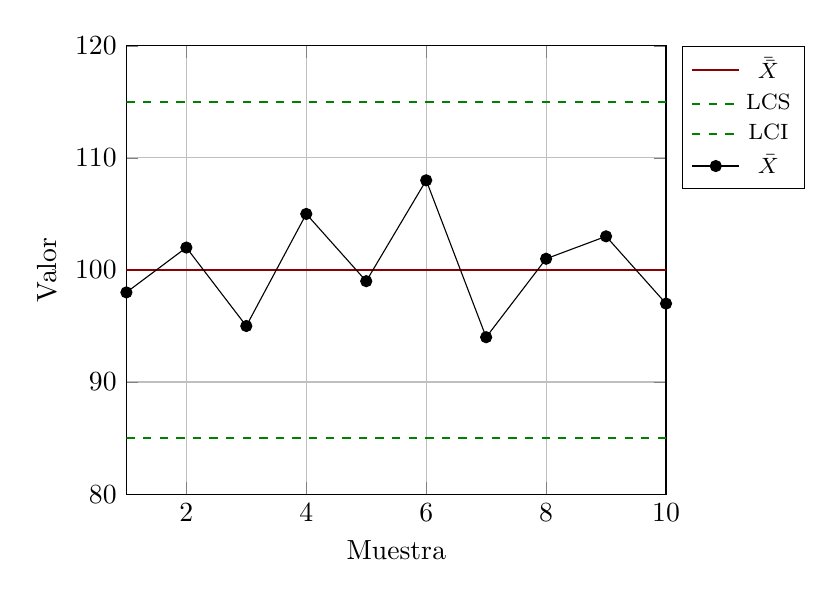
\begin{tikzpicture}
\begin{axis}[
    xlabel={Muestra}, xmin=1, xmax=10,
    ylabel={Valor}, ymin=80, ymax=120,
    grid=major,
    legend pos=outer north east
]

\addplot[DarkRed, solid, thick] coordinates {(1,100) (10,100)};
\addlegendentry{\footnotesize $\bar{\bar{X}}$}

\addplot[Green, dashed, thick] coordinates {(1,115) (10,115)};
\addlegendentry{\footnotesize LCS}
\addplot[Green, dashed, thick] coordinates {(1,85) (10,85)};
\addlegendentry{\footnotesize LCI}

\addplot[black, mark=*] coordinates {
    (1,98) (2,102) (3,95) (4,105) (5,99) 
    (6,108) (7,94) (8,101) (9,103) (10,97)
};
\addlegendentry{\footnotesize $\bar{X}$}

\end{axis}
\end{tikzpicture}